\documentclass[aspectratio=169]{beamer}
\usepackage[utf8]{inputenc}
\usefonttheme{serif}
\usetheme{boxes}
\setbeamertemplate{frametitle}[default][center]
\setbeamersize{text margin right=20mm, text margin left=20mm} 
\addtobeamertemplate{frametitle}{\vskip1cm}{}
\setbeamertemplate{navigation symbols}{}

%% absolute positioning
\usepackage[absolute,overlay]{textpos}
\usepackage{mathrsfs} % https://www.ctan.org/pkg/mathrsfs
%Information to be included in the title page:
\title{\bf\LARGE Papers We Love \color{gray}{Milano} \#4}
\subtitle{Partial Computation of Programs\\[5pt] (Futamura 1984)}
\author{Edoardo Vacchi}
% \institute{Overleaf}
\date{19th February 2020}
 
 
\begin{document}
 
\frame{\titlepage}

\begin{frame}{ex}
    Let us have a computation $f$ of two parameters $k$, $u$
    \[
        f(k,u)
    \]
    Now suppose that $f$ is often called with $k=5$; 
    
    we may define the program $f_5(u)$ by substituting $5$ for $k$ in $f$ 
    and doing all possible computation based upon value $5$.

    Partial evaluation is the process of rewriting $f(5,u)$
\end{frame}
 


\begin{frame}

    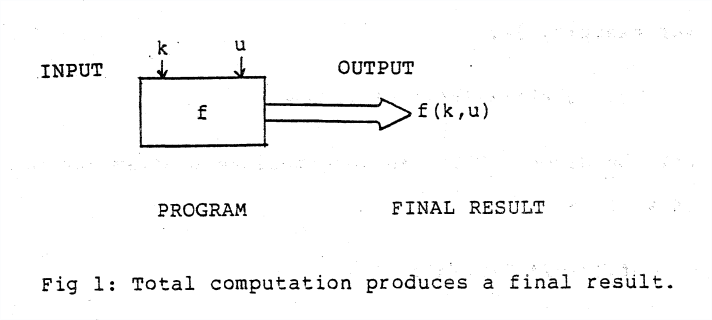
\includegraphics[width=\textwidth]{imgs/fig1.png}

\end{frame}
 


\begin{frame}

    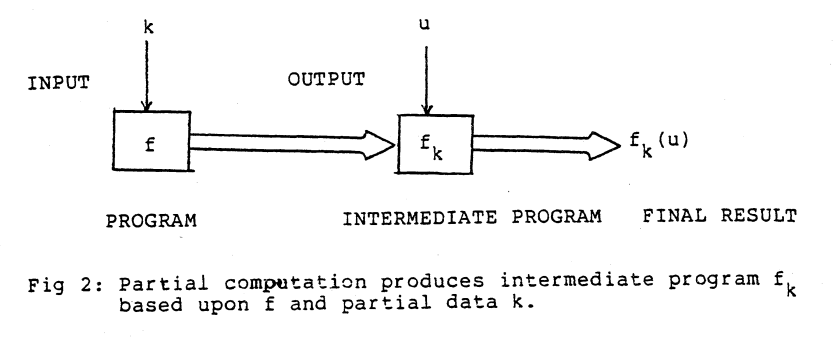
\includegraphics[width=\textwidth]{imgs/fig2.png}

\end{frame}
 
\begin{frame}
Consider $f$

    \[
        f(k,u) \triangleq k \cdot ( k \cdot (k+1) + u + 1) + u\cdot u
    \]

now let $k=2$, we can write $f_2$ as follows

    \[
        f_2(u) \triangleq 2 \cdot (7+u) + u\cdot u    
    \]

because $f(2,u) = f_2(u)$ for any value of $u$, 
the following equation holds for $f_k$ and $f$



    \begin{equation}
        f_k(u)=f(k,u)
    \end{equation}

And we call it \textit{a projection of $f$ at $k$}

\end{frame}

\begin{frame}{Partial Evaluator}

A partial computation procedure may be a computer program $\alpha$
called \textit{a projection machine}, \textit{partial computer} 
or \textit{partial evaluator}.

\begin{equation}
    \alpha(f,k) = f_k
\end{equation}
\end{frame}


\begin{frame}{Basic Equation of Partial Evaluation}

Non consider $\alpha_f$, the partial evaluation of $\alpha$ at $f$; then:

\begin{eqnarray*}
            &\alpha_f(k) &= \alpha(f,k)\\
            &\alpha(f,k) &= f_k
\end{eqnarray*}

therefore:
\begin{equation}
       \alpha_k =f_k 
\end{equation}
\end{frame}


\begin{frame}{First Equation of Partial Computation}

    
An \textit{interpreter} $\mathcal{I}$ is a program to perform
specified computations that analyze the meanings of a given program, 
say $\mathcal{P}$, based upon given data, say $\mathcal{D}$. 

Thus, 
running a program by intepreter means performing $\mathcal{I}(\mathcal{P}, \mathcal{D})$


A \textit{compiler}, say $\mathcal{C}$, translates a source program
say $\mathcal{P}$, to an object program $\mathcal{C}(\mathcal{P})$

This produces the following equation:

\[
    \mathcal{C}(\mathcal{P})(\mathcal{D}) = \mathcal{I}(\mathcal{P},\mathcal{D})
\]

while $ \mathcal{I}_{\mathcal{P}} =  \alpha(\mathcal{I},\mathcal{P}) $

\begin{equation}
\mathcal{I}_{\mathcal{P}} =  \mathcal{C}(\mathcal{P})
\end{equation}


\end{frame}


\begin{frame}{Second Equation of Partial Computation}

    
    \begin{equation}
    \alpha_\mathcal{I}(\mathcal{P}) =  \mathcal{I}_\mathcal{P}
    \end{equation}
    
    
\end{frame}

\begin{frame}{Third Equation of Partial Computation}

    
    \begin{equation}
    \alpha_\alpha(\mathcal{I}) =  \alpha_\mathcal{I}
    \end{equation}
    
    $\alpha_\alpha$ is a compiler-compiler
    
\end{frame}


\begin{frame}{Fourth Equation of Partial Computation}

    \[
        \alpha_\alpha(\alpha)=\alpha_\alpha    
    \]

    this means that $\alpha_\alpha$ is an $\alpha$-language compiler.
    Therefore $\alpha_\alpha(f)$ is an object program of $f$
    thus we get the equation: 
    
    \begin{equation}
    \alpha_\alpha(f)(k) =  f_k
    \end{equation}
    
    $\alpha_\alpha$ is a compiler-compiler
    
\end{frame}
     
\end{document}
    